\documentclass{standalone}
\usepackage{tikz}
\usetikzlibrary{calc}

\usepackage{tikz}
\usetikzlibrary{decorations.markings}
\usetikzlibrary{math}

\newcommand\getLength[4]{sqrt((#1-#3)*(#1-#3) + (#2-#4)*(#2-#4))}


\begin{document}

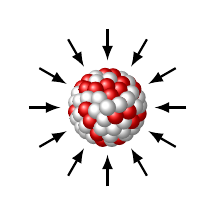
\begin{tikzpicture}
\tikzset{
    pics/proton/.style={code={\shade[ball color=red] circle (3pt);}},
    pics/neutron/.style={code={\shade[ball color=white] circle (3pt);}},
    pics/nucleussmall/.style={code={%
        \pgfmathdeclarerandomlist{nucleon}{{proton}{proton}{neutron}{neutron}{neutron}}
        \pgfmathsetseed{#1+1}
        \foreach \A/\R in {8/0.2, 5/0.13, 1/0}{
        \pgfmathsetmacro{\S}{360/\A}
            \foreach \B in {0,\S,...,360}{
                \pgfmathrandomitem{\C}{nucleon}
                \pic at ($(\B+2*\A+5*rnd:\R)$) {\C}; } }} },
    pics/nucleusbig/.style={code={%
        \pgfmathdeclarerandomlist{nucleon}{{proton}{proton}{neutron}{neutron}{neutron}}
        \pgfmathsetseed{#1+1}
        \foreach \A/\R in {24/0.4, 24/0.3, 24/0.2, 13/0.35, 11/0.27, 6/0.15, 1/0}{
        \pgfmathsetmacro{\S}{360/\A}
            \foreach \B in {0,\S,...,360}{
                \pgfmathrandomitem{\C}{nucleon}
                \pic at ($(\B+2*\A+5*rnd:\R)$) {\C}; } }} },
    pics/nucleusbiggest/.style={code={%
        \pgfmathdeclarerandomlist{nucleon}{{proton}{proton}{neutron}{neutron}{neutron}}
        \pgfmathsetseed{#1+1}
        \foreach \A/\R in {24/0.5, 24/0.4, 24/0.3, 24/0.2, 13/0.47, 15/0.44, 13/0.37, 11/0.27, 6/0.15, 1/0}{
        \pgfmathsetmacro{\S}{360/\A}
            \foreach \B in {0,\S,...,360}{
                \pgfmathrandomitem{\C}{nucleon}
                \pic at ($(\B+2*\A+5*rnd:\R)$) {\C}; } }} },
    }
\pic at (0,0) {nucleusbig};


% Number of arrows
\tikzmath{
    \n = 12;
    \step = 360/\n;
    \radius = 0.8;
    \radiuss = 0.4;
    \rotationalSpeed = 1.0;
}

\foreach \x in {1,...,\n} {

    % Sets up the line elements with correct rotations    
    \tikzmath{
        \xone = \radius*cos(\x*\step);
        \xtwo = \radius*sin(\x*\step);
        \yone = \radius*cos(\x*\step) + \radiuss*cos(\x*\rotationalSpeed*\step);
        \ytwo = \radius*sin(\x*\step) + \radiuss*sin(\x*\step*\rotationalSpeed);
        \R = \getLength{\xone}{\xtwo}{\yone}{\ytwo};
    }

    % Draws the vector
    \draw[thick,-latex] 
    ({\yone - 0.5*(\yone-\xone)},
    {\ytwo - 0.5*(\ytwo-\xtwo)})
    --
    ({\xone - 0.5*(\yone-\xone)},
    {\xtwo - 0.5*(\ytwo-\xtwo)})
    ;
}


\end{tikzpicture}
\end{document}